\documentclass{article}

\usepackage{hyperref}
\usepackage{graphicx}

\title{Quality Threshold Clustering}
\author{Loconte Lorenzo, M. 683124}

\begin{document}
	\maketitle
	\section{Introduzione}
	In statistica, il \textbf{clustering} è un insieme di tecniche volte
	alla selezione e raggruppamento di elementi omogenei in un insieme di
	dati. Le tecniche di clustering si basano su misure relative alla
	somiglianza degli elementi. Gli algoritmi di clustering raggruppano gli
	elementi sulla base della loro distanza reciproca.

	\section{QT-Clustering}
	\textbf{QT-Clustering} è composto da due applicazioni, un client ed un
	server. Lo scopo del progetto è permettere a molteplici client di
	eseguire un algoritmo di clustering su un server utlizzando come
	sorgente dei dati un database MySQL.

	\subsection{Server}
	Il server si occupa principalmente di accettare le richieste dei client.
	Esso esegue l'algoritmo di clustering vero e proprio utilizzando come
	sorgente dei dati una tabella (specificata dal client) di un database
	MySQL. Le funzionalità del server sono le seguenti:
	\begin{itemize}
		\item Inizializzare il server su una porta arbitraria.
		\item Capacità di gestire le richieste di molteplici client in
		contemporanea.
		\item Leggere il contenuto di una tabella di una base di dati
		indipendentemente dal numero di attributi e dal numero di tuple.
		\item Eseguire l'algoritmo di \textbf{Quality Threshold
		clustering} usando un raggio arbitrario su un numero indefinito
		di tuple.
		\item Fare operazioni di \textbf{Principal Component Analysis}
		per estrarre dalle tuple le componenti principali.
		\item Salvare su file l'esito della computazione come cache.
		\item Restituire ai client l'esito della computazione.
	\end{itemize}

	\subsection{Client}
	Il client è fornito di una interfaccia grafica che permette ad un'utente
	di connettersi al server e selezionare la fonte dei dati su cui eseguire
	l'algoritmo di clustering. Inoltre il client si occupa di rappresentare
	in forma grafica i cluster o i centroidi all'interno di un grafico
	bidimensionale.

	\subsection{Estensione}
	L'estensione principale rispetto al progetto originale è la grafica per
	l' applicazione client. Un'altra estensione, sempre a supporto della
	grafica, è costituita da un'algoritmo di \textbf{Principal Component
	Analysis}.

	\subsubsection{Grafica}
	La grafica per l'applicazione client è stata scritta utilizzando le
	\textbf{JavaFX}.

	\subsubsection{Principal Component Analysis}
	La \textbf{Principal Component Analysis} (da adesso abbreviato con
	\textbf{PCA}) è una tecnica appartenente alla statistica multivariata
	usata per estrarre da un insieme di dati N dimensionali M componenti
	principali in modo tale da ridurre il numero di dimensioni dello spazio
	in cui si trovano i dati. L'esigenza di fare ciò nasce dal fatto che è
	molto difficile rappresentare tuple in uno spazio a più di tre
	dimensioni. Pertanto, tramite algoritmi di \textbf{PCA}, è possibile
	proiettare i dati in uno spazio tridimensionale (o anche bidimensionale)
	che sia trattabile e soprattuto rappresentabile. Ovviamente la scelta
	degli assi di proiezione non è arbitraria, infatti punti molto distanti
	tra loro in uno spazio N dimensionale possono ritrovarsi ad essere molto
	vicini in uno spazio M dimensionale (con M \textless N). Generalmente
	si scelgono gli assi di proiezione in modo tale che il campione
	proiettato abbia varianza massima. L'algoritmo di \textbf{PCA}
	implementato è il seguente:
	\begin{enumerate}
		\item Si trasforma il campione misto (numerico e discreto) in
		un campione numerico.
		\item Si standardizza il campione.
		\item Si calcola la matrice di covarianza del campione.
		\item Si calcolano autovalori ed autovettori della matrice di
		covarianza.
		\item Si scelgono come assi di proiezione gli autovettori
		associati agli autovalori più grandi.
		\item Si proietta il campione standardizzato sugli assi di
		proiezione.
	\end{enumerate}
	Si tenga presente che questa procedura sacrifica parte dell'informazione
	del campione originario. Il calcolo delle componenti principali è
	effettuato dal server al termine dell'esecuzione dell'algoritmo di
	clustering. E' compito del client poi disegnare sullo scatter-plot
	i punti. Come libreria per l'algebra lineare è stata usata la libreria
	\href{http://la4j.org}{\textbf{la4j}}.

	\section{Manuale utente}

	\subsection{Client}
	\begin{figure}[h]
		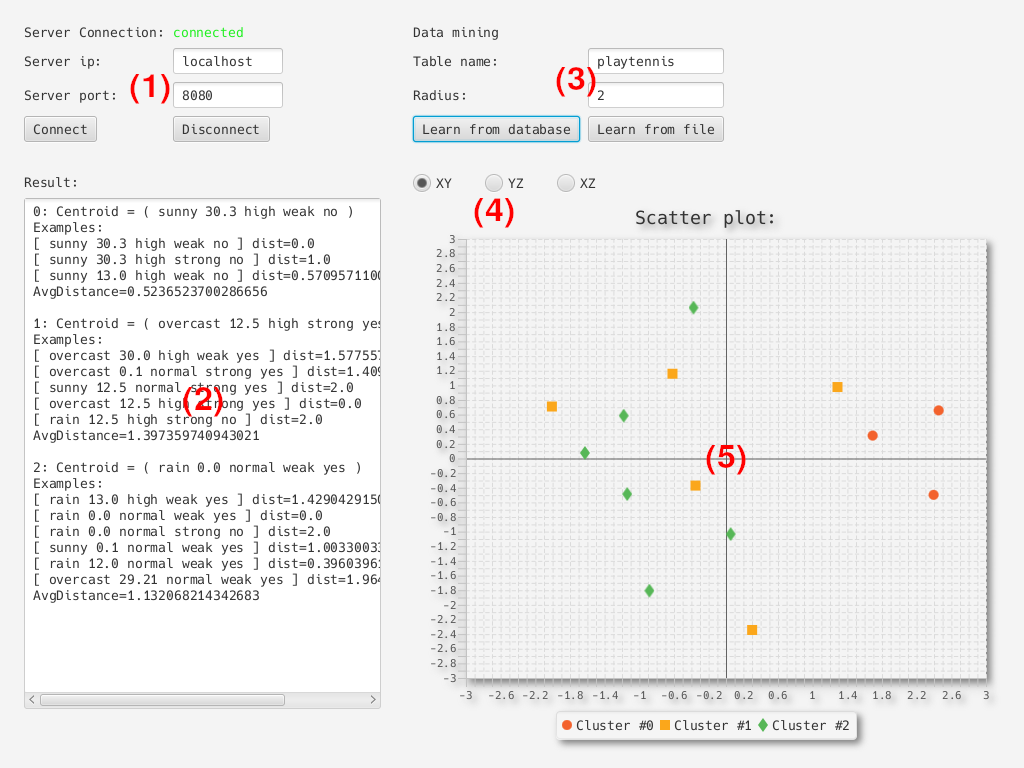
\includegraphics[width=\linewidth]{windowform.png}
		\caption{Il form della finestra del client}
	\end{figure}
	\begin{enumerate}
		\item L'utente sceglie IP e porta del server a cui desidera connettersi.
		Un'etichetta posta in cima al form comunica lo stato della connessione.
		Se IP o porta risultano non validi si aprirà una finestra di errore.
		L'utente può scegliere, attraverso i pulsanti, di connettersi o
		disconnettersi. Quando si è disconnessi e si prova a fare un'operazione
		verrà mostrato a video un errore.
		\item Il risultato, in forma testuale, dell'operazione di data mining.
		Vengono mostrati i cluster e/o i centroidi e, per ogni cluster, viene
		mostrata anche la distanza media delle tuple dal centroide.
		\item L'utente sceglie nome della tabella del database e raggio da
		utilizzare. Se la tabella risulta non presente nel database oppure il
		raggio risulta non valido verrà mostrato a video un errore. L'utente
		può scegliere se eseguire l'algoritmo di mining partendo da una tabella
		del database oppure leggere da file. Se il raggio risulta talmente
		grande tale che il risultato della computazione è un unico cluster
		oppure il file non è presente sul server allora verrà mostrato a
		video un errore.
		\item L'utente sceglie uno dei tre piani di proiezione dei dati:
		XY, YZ oppure XZ. In base alla scelta cambierà lo stato dello scatter
		plot. Si tenga presente che si perde parte dell'informazione delle
		tuple originarie.
		\item Lo scatter plot su cui vengono rappresentati i dati. Ogni cluster
		(o centroide) possiede un colore ed una etichetta diversa. Al di sotto
		della griglia è presente una legenda.
	\end{enumerate}

	\subsection{Server}
	Di default, la porta utilizzata dal server è la \textbf{8080}.
	Tuttavia, al momento dell'esecuzione è possibile specificare
	la porta da utilizzare da riga di comando come parametro di
	input al file \textit{Bash/Bat}. Verrà stampato un errore
	se il formato della porta non è valido oppure se la porta è
	occupata.

	\section{Note tecniche}
	Per il progetto è stato utilizzato lo strumento \textbf{git}. Inoltre
	il progetto è stato hostato su un repository remoto privato su
	\href{https://github.com}{\textbf{GitHub}}. Come strumento di build
	system e gestione delle dipendenze è stato utilizzato \textbf{Gradle}.
	In questo modo si ha la completa indipendenza dall'IDE che si intende
	utilizzare. 
	Durante lo sviluppo sono stati utilizzati i seguenti strumenti:
	\begin{itemize}
		\item \textit{JUnit 4.12}, per i casi di test.
		\item \textit{JaCoCo}, per la copertura dei casi di test.
		\item \textit{Checkstyle}, per verificare lo stile.
	\end{itemize}
	Sono stati scritti casi di test esclusivamente per il \textit{server}
	dato che il client è costituito principalmente da codice per la UI.	
	Attualmente la copertura dei casi di test è pari al \textbf{74\%}.
	I vari reports (\textit{Javadoc}, \textit{JUnit}, \textit{JaCoCo} e
	\textit{Checkstyle}) si trovano all'interno di
	\textit{/qt-clustering/reports}.
	I diagrammi delle classi e dei packages si trovano all'interno di
	\textit{/qt-clustering/documentation}.

	\subsection {Guida per l'installazione}
	I file per la distribuzione (file \textit{Bash/Bat} e
	\textit{.jar}) sia per il client che per il server si trovano in
	\textit{/qt-clustering/distributions}.
	Per eseguire il server è necessario aver installato MySQL.
	Dopodichè bisogna accertarsi che il servizo di MySQL sia in
	esecuzione. Bisogna poi inizializzare il database MySQL eseguendo lo
	script \textit{mapdb.sql} presente nella cartella
	\textit{/qt-clustering/distributions/server}.
	Lo script SQL contiene le istruzioni per creare un database \textit{MapDB}
	contenente una tabella di esempio chiamata \textbf{playtennis}
	ed un'altra tabella chiamata \textbf{test} richiesta per
	l'esecuzione dei casi di test. Inoltre esso crea un nuovo utente
	(se non presente) chiamato \textit{MapUser} con diritti di accesso
	per il database \textit{MapDB}.

	\subsection {Importare il progetto con Eclipse}
	Attraverso il tool \textit{Gradle} è possibile, da riga di comando,
	compilare ed eseguire sia il client sia il server. Inoltre è anche
	possibile eseguire i casi di test e generare la documentazione
	\textit{Javadoc}.
	In alternativa è possibile importare il progetto con
	Eclipse seguendo i seguenti passi:
	\begin{enumerate}
		\item Importare il progetto come progetto \textit{Gradle}:
			\textit{File \textgreater Import ... \textgreater Gradle
			\textgreater Existing Gradle Project}
		\item Selezionare la root directory del progetto
		\item Cliccare su \textit{Finish}
	\end{enumerate}
	Verranno così importati due progetti, uno per il \textit{server} e uno
	per il \textit{client}. Gradle scaricherà automaticamente tutte le
	dipendenze necessarie. Per eseguire il \textit{client/server} basterà
	aprire la finestra dei \textit{Gradle Tasks}, selezionare il progetto,
	e cliccare su \textit{application \textgreater run}. Se la finestra
	\textit{Gradle Tasks} non è presente allora è necessario aprirla
	selezionando \textit{Window \textgreater Show View \textgreater Other...
	\textgreater Gradle \textgreater Gradle Tasks}. Sempre dalla stessa
	finestra \textit{Gradle Tasks} è possibile fare altre operazioni, tra
	cui la generazione del \textit{Javadoc} e l'esecuzione dei casi di test.
\end{document}

